\documentclass[aspectratio=169,xcolor=dvipsnames]{beamer}
\usetheme{Madrid}
\usecolortheme{seahorse}
\usepackage{amsmath,amssymb,booktabs,hyperref,listings,tikz}
\lstset{
  basicstyle=\small\ttfamily,
  keywordstyle=\color{blue}\bfseries,
  commentstyle=\color{OliveGreen},
  stringstyle=\color{red},
  frame=single,
  breaklines=true
}

\title[Algorithms -- Week 2]{\textbf{Design and Analysis of Algorithms}\\
\large Week 2: Asymptotic Notation and Complexity Classes}
\subtitle{TOAE209/TOAH209 -- Foreign Trade University}
\author{Department of Technology \& Data Science}
\date{Semester 2024--2025}

\AtBeginSection[]{
  \begin{frame}<beamer>{Outline}
    \tableofcontents[currentsection]
  \end{frame}
}

\begin{document}

\begin{frame}
  \titlepage
\end{frame}

\begin{frame}{Outline}
  \tableofcontents
\end{frame}

\section{Why This Week Matters}
\begin{frame}{Why Formal Notation Matters}
  \begin{itemize}
    \item We need a way to compare algorithms without tying the answer to one machine
    \item Constant factors depend on language, compiler, CPU, and memory layout
    \item Growth rate is the part that survives scale
    \item Asymptotic notation is the language for that growth rate
  \end{itemize}
  \begin{exampleblock}{Running idea}
    We will keep one campus example in mind: a student-record system that must search, sort, and validate data as the number of records grows.
  \end{exampleblock}
\end{frame}

\begin{frame}{What the Week Covers}
  \begin{enumerate}
    \item How to talk about growth with $O$, $\Omega$, and $\Theta$
    \item How to prove bounds instead of guessing them
    \item How to compare common growth classes
    \item How to classify problems as P, NP, NP-hard, or undecidable
    \item Why reductions matter in practice
  \end{enumerate}
  \begin{block}{Goal}
    By the end, you should be able to read an algorithm and say what dominates its cost, why, and what class of problem it belongs to.
  \end{block}
\end{frame}

\begin{frame}{The Running Example}
  Suppose the university stores registration records:
  \begin{itemize}
    \item each record has a student ID, course code, and timestamp
    \item staff want to search by ID
    \item the system may sort records by ID or time
    \item the system may detect duplicates or conflicts
  \end{itemize}
  \begin{alertblock}{Question}
    If the record count doubles, which operations get twice as slow, which get only slightly slower, and which become much worse?
  \end{alertblock}
\end{frame}

\begin{frame}{Same Code, Different Scale}
  \begin{itemize}
    \item 50 records: almost any solution feels fast
    \item 5,000 records: inefficient loops start to show
    \item 500,000 records: the wrong algorithm becomes unusable
  \end{itemize}
  \begin{exampleblock}{Lesson}
    Big-O is not about tiny inputs. It is about what survives when the dataset is large enough to expose the algorithm's structure.
  \end{exampleblock}
\end{frame}

\begin{frame}{Input Size Is the Real Variable}
  \begin{itemize}
    \item For search, $n$ is the number of records
    \item For sorting, $n$ is the number of items to order
    \item For graph problems, $n$ may be vertices and $m$ edges
    \item For strings, $n$ is the length of the text or pattern
  \end{itemize}
  \begin{block}{Good habit}
    Always ask: what exactly does $n$ count in this problem?
  \end{block}
\end{frame}

\begin{frame}{A Simple Cost Model}
  \begin{itemize}
    \item Count primitive operations, comparisons, and assignments
    \item Ignore hardware details unless they change the dominant term
    \item Treat memory usage separately from running time
  \end{itemize}
  \begin{exampleblock}{We usually ask}
    How many basic steps does the algorithm perform as a function of $n$?
  \end{exampleblock}
\end{frame}

\begin{frame}{What Asymptotics Keeps}
  \begin{itemize}
    \item the highest-order term
    \item the structure of loops and recursion
    \item the difference between linear, quadratic, and exponential growth
  \end{itemize}
  \begin{block}{Example}
    $3n^2 + 12n + 7$ behaves like $n^2$ for large $n$.
  \end{block}
\end{frame}

\begin{frame}{What Asymptotics Ignores}
  \begin{itemize}
    \item constant multipliers
    \item lower-order terms
    \item implementation details that do not change the dominant growth rate
  \end{itemize}
  \begin{alertblock}{Important}
    Ignoring constants does not mean constants are useless. They still matter for practical break-even points.
  \end{alertblock}
\end{frame}

\begin{frame}{A First Timing Thought Experiment}
  \begin{itemize}
    \item Algorithm A: $1000n$ steps
    \item Algorithm B: $n^2$ steps
  \end{itemize}
  \begin{block}{For small $n$}
    B may be faster because the constant in A is large.
  \end{block}
  \begin{block}{For large $n$}
    A wins because linear growth beats quadratic growth.
  \end{block}
\end{frame}

\section{Big-O}
\begin{frame}{Big-O: Formal Definition}
  \begin{block}{Definition}
    $f(n) = O(g(n))$ if there exist constants $c > 0$ and $n_0$ such that
    \[
      0 \le f(n) \le c \, g(n) \quad \text{for all } n \ge n_0.
    \]
  \end{block}
  \begin{itemize}
    \item Big-O is an asymptotic upper bound
    \item It says $f$ does not grow faster than a constant multiple of $g$
  \end{itemize}
\end{frame}

\begin{frame}{Big-O: Intuition}
  \begin{itemize}
    \item Think of a ceiling above the function
    \item The ceiling only needs to work after some threshold $n_0$
    \item What happens for tiny inputs is not important to the definition
  \end{itemize}
  \begin{exampleblock}{Reading}
    "$f(n)$ is $O(g(n))$" means "$f$ grows no faster than $g$ up to a constant factor."
  \end{exampleblock}
\end{frame}

\begin{frame}{Big-O Example: Linear Search}
  \begin{itemize}
    \item The algorithm checks each record until it finds the target or reaches the end
    \item Worst case: the target is absent or last
    \item Number of comparisons is at most $n$
  \end{itemize}
  \begin{block}{Conclusion}
    Linear search is $O(n)$.
  \end{block}
\end{frame}

\begin{frame}[fragile]{Big-O Example: Nested Loop}
  \begin{lstlisting}[language=Python]
count = 0
for i in range(n):
    for j in range(n):
        count += 1
  \end{lstlisting}
  \begin{itemize}
    \item Inner statement runs $n \cdot n$ times
    \item Dominant term is $n^2$
  \end{itemize}
  \begin{block}{Conclusion}
    The loop is $O(n^2)$.
  \end{block}
\end{frame}

\begin{frame}{Big-O Example: One Heavy and One Light Term}
  \[
    3n^2 + 40n + 17
  \]
  \begin{itemize}
    \item the quadratic term dominates
    \item the linear and constant terms eventually vanish in comparison
  \end{itemize}
  \begin{block}{Result}
    $3n^2 + 40n + 17 = O(n^2)$.
  \end{block}
\end{frame}

\begin{frame}{Proving an Upper Bound}
  To prove $f(n) = O(g(n))$:
  \begin{enumerate}
    \item choose a candidate $g(n)$
    \item find constants $c$ and $n_0$
    \item show $f(n) \le c g(n)$ for all $n \ge n_0$
  \end{enumerate}
  \begin{exampleblock}{Example}
    For $3n^2 + 40n + 17$, one valid choice is $c = 60$ and $n_0 = 1$.
  \end{exampleblock}
\end{frame}

\begin{frame}{Big-O Non-Example}
  \begin{itemize}
    \item $n^2$ is not $O(n)$
    \item the ratio $n^2 / n = n$ grows without bound
    \item no constant multiple of $n$ can keep up with $n^2$
  \end{itemize}
  \begin{alertblock}{Takeaway}
    A claim can fail because the proposed ceiling is too small.
  \end{alertblock}
\end{frame}

\begin{frame}{Upper Bound Versus Tight Bound}
  \begin{itemize}
    \item $2n = O(n^2)$ is true
    \item but it is not useful
    \item $2n = O(n)$ is the useful statement
  \end{itemize}
  \begin{block}{Rule of thumb}
    Use the tightest bound you can justify.
  \end{block}
\end{frame}

\begin{frame}{Big-O Rules You Will Use Often}
  \begin{itemize}
    \item $O(f) + O(g) = O(\max(f,g))$
    \item $O(cf) = O(f)$ for any constant $c > 0$
    \item $O(f) \cdot O(g) = O(fg)$
  \end{itemize}
  \begin{exampleblock}{Interpretation}
    When you combine parts of an algorithm, keep only the dominating term.
  \end{exampleblock}
\end{frame}

\begin{frame}{Logs in Big-O}
  \begin{itemize}
    \item $\log_a n$ and $\log_b n$ differ only by a constant factor
    \item therefore they are the same asymptotic class
    \item logarithms grow much slower than polynomials
  \end{itemize}
  \begin{block}{Useful fact}
    $\log^k n = o(n^\epsilon)$ for any fixed $k$ and $\epsilon > 0$.
  \end{block}
\end{frame}

\begin{frame}{Big-O and Recursion Preview}
  \begin{itemize}
    \item recursion often leads to recurrence relations
    \item each recursive call contributes a subproblem
    \item the total cost is the sum of all levels
  \end{itemize}
  \begin{block}{Week 3 link}
    In divide and conquer, Big-O will be combined with recurrences.
  \end{block}
\end{frame}

\section{Omega and Theta}
\begin{frame}{Big-Omega: Lower Bound}
  \begin{block}{Definition}
    $f(n) = \Omega(g(n))$ if there exist constants $c > 0$ and $n_0$ such that
    \[
      0 \le c\,g(n) \le f(n) \quad \text{for all } n \ge n_0.
    \]
  \end{block}
  \begin{itemize}
    \item Big-Omega is a floor
    \item it says $f$ grows at least as fast as a constant multiple of $g$
  \end{itemize}
\end{frame}

\begin{frame}{Big-Theta: Tight Bound}
  \begin{block}{Definition}
    $f(n) = \Theta(g(n))$ if $f(n) = O(g(n))$ and $f(n) = \Omega(g(n))$.
  \end{block}
  \begin{itemize}
    \item Theta means both an upper and a lower bound
    \item It is the most informative asymptotic statement when it is available
  \end{itemize}
\end{frame}

\begin{frame}{Theta Example}
  \[
    2n^2 + 3n + 1
  \]
  \begin{itemize}
    \item it is at most a constant multiple of $n^2$
    \item it is also at least a constant multiple of $n^2$
  \end{itemize}
  \begin{block}{Conclusion}
    $2n^2 + 3n + 1 = \Theta(n^2)$.
  \end{block}
\end{frame}

\begin{frame}{Theta Example: Linear Search}
  \begin{itemize}
    \item best case: the target is first
    \item worst case: the target is absent or last
    \item in the worst case, the number of checks grows linearly
  \end{itemize}
  \begin{block}{Worst-case cost}
    Linear search is $\Theta(n)$ in the worst case.
  \end{block}
\end{frame}

\begin{frame}{Theta Versus Big-O}
  \begin{itemize}
    \item $O(g)$ alone only says "no worse than"
    \item $\Theta(g)$ says "same growth rate up to constants"
    \item if you know both an upper and a lower bound, report $\Theta$
  \end{itemize}
  \begin{exampleblock}{Example}
    $n$ is $O(n^2)$, but only $\Theta(n)$ gives the right story.
  \end{exampleblock}
\end{frame}

\begin{frame}{Little-o and Little-omega}
  \begin{block}{Little-o}
    $f(n) = o(g(n))$ if $\lim_{n \to \infty} \frac{f(n)}{g(n)} = 0$.
  \end{block}
  \begin{block}{Little-omega}
    $f(n) = \omega(g(n))$ if $\lim_{n \to \infty} \frac{f(n)}{g(n)} = \infty$.
  \end{block}
\end{frame}

\begin{frame}{Limit Test Examples}
  \begin{itemize}
    \item $n = o(n^2)$ because $n/n^2 = 1/n \to 0$
    \item $n \log n = o(n^{1.5})$ because the polynomial wins
    \item $n^2 = \omega(n \log n)$ because the ratio diverges
  \end{itemize}
  \begin{block}{Use carefully}
    Limits are a fast proof tool when the algebra is clean.
  \end{block}
\end{frame}

\begin{frame}{A Useful Identity}
  \[
    \log_a n = \frac{\log_b n}{\log_b a}
  \]
  \begin{itemize}
    \item changing the log base only multiplies by a constant
    \item Big-O ignores that constant
  \end{itemize}
  \begin{exampleblock}{Conclusion}
    All log bases are equivalent asymptotically.
  \end{exampleblock}
\end{frame}

\begin{frame}{Theta From Two Sides}
  To prove $f(n)=\Theta(g(n))$:
  \begin{enumerate}
    \item prove $f(n)=O(g(n))$
    \item prove $f(n)=\Omega(g(n))$
  \end{enumerate}
  \begin{block}{Example strategy}
    For a polynomial, bound by the highest-order term from above and below.
  \end{block}
\end{frame}

\begin{frame}{Common Misreadings}
  \begin{itemize}
    \item $O(n^2)$ does not mean exactly quadratic
    \item $\Theta(n)$ does not mean one step per input item in code
    \item asymptotic notation describes growth, not line-by-line syntax
  \end{itemize}
  \begin{alertblock}{Warning}
    A good proof uses the definition, not intuition alone.
  \end{alertblock}
\end{frame}

\section{Proof Toolkit}
\begin{frame}{How to Prove an Asymptotic Bound}
  \begin{itemize}
    \item isolate the dominant term
    \item compare everything to a known function
    \item choose constants explicitly
    \item state the threshold $n_0$
  \end{itemize}
  \begin{block}{Template}
    "For all $n \ge n_0$, we have $f(n) \le c g(n)$."
  \end{block}
\end{frame}

\begin{frame}{Bounding by the Largest Term}
  \[
    5n^3 + 100n^2 + n + 1000
  \]
  \begin{itemize}
    \item the cubic term dominates
    \item the others are lower-order
  \end{itemize}
  \begin{block}{Result}
    This expression is $\Theta(n^3)$.
  \end{block}
\end{frame}

\begin{frame}{Geometric Series Pattern}
  \[
    1 + 2 + 4 + \cdots + 2^{k}
  \]
  \begin{itemize}
    \item the last term dominates the sum
    \item the total is less than twice the last term
  \end{itemize}
  \begin{block}{Typical conclusion}
    Geometric sums are the same order as their largest term.
  \end{block}
\end{frame}

\begin{frame}{A Loop Becomes a Sum}
  \begin{itemize}
    \item a loop with changing bounds is usually a summation
    \item count one iteration per inner statement
    \item simplify the sum into a closed form
  \end{itemize}
  \begin{exampleblock}{Example}
    \[
      \sum_{i=0}^{n-1} (n-i-1) = \frac{n(n-1)}{2}
    \]
  \end{exampleblock}
\end{frame}

\begin{frame}{Pair Counting}
  \begin{itemize}
    \item many quadratic algorithms count pairs
    \item the number of unordered pairs is $\binom{n}{2}$
    \item this equals $n(n-1)/2$
  \end{itemize}
  \begin{block}{Interpretation}
    When you compare every element with every later element, expect $\Theta(n^2)$.
  \end{block}
\end{frame}

\begin{frame}{Why the First Few Terms Do Not Matter}
  \begin{itemize}
    \item constants matter for benchmarking
    \item constants do not matter for asymptotic classification
    \item lower-order terms vanish after the threshold
  \end{itemize}
  \begin{exampleblock}{Example}
    $1000000n + n^2$ is eventually dominated by $n^2$.
  \end{exampleblock}
\end{frame}

\begin{frame}{Proof by Direct Inequality}
  To show $n \log n = O(n^{1.5})$:
  \begin{itemize}
    \item divide both sides by $n$
    \item compare $\log n$ with $\sqrt{n}$
    \item note that logarithms grow more slowly than any positive power
  \end{itemize}
  \begin{block}{Conclusion}
    The polynomial term wins.
  \end{block}
\end{frame}

\begin{frame}{How to Negate a Claim}
  To disprove $f(n)=O(g(n))$:
  \begin{itemize}
    \item look at the ratio $f(n)/g(n)$
    \item if it becomes arbitrarily large, no constant works
  \end{itemize}
  \begin{exampleblock}{Example}
    $n^2$ is not $O(n)$ because $n^2/n = n \to \infty$.
  \end{exampleblock}
\end{frame}

\begin{frame}{A Practical Proof Pattern}
  \begin{enumerate}
    \item write the exact count
    \item simplify the count
    \item identify the dominant term
    \item convert to $O$, $\Omega$, or $\Theta$
  \end{enumerate}
  \begin{block}{Why it helps}
    This makes the proof checkable by another person.
  \end{block}
\end{frame}

\begin{frame}{An Inductive View of Bounds}
  \begin{itemize}
    \item induction is useful when a problem builds on smaller inputs
    \item it is common for recurrences and recursive algorithms
    \item we will use it more heavily in divide and conquer
  \end{itemize}
  \begin{exampleblock}{Connection}
    Recurrence solving is the next natural step after asymptotic notation.
  \end{exampleblock}
\end{frame}

\begin{frame}{Fast Growth Rules}
  \begin{itemize}
    \item if $a > 1$, then $a^n$ beats every polynomial
    \item factorial growth beats exponentials
    \item logarithms are the slowest standard family we use often
  \end{itemize}
  \begin{block}{Mental ladder}
    $\log n \ll n \ll n \log n \ll n^2 \ll 2^n \ll n!$
  \end{block}
\end{frame}

\section{Growth Comparison}
\begin{frame}{The Growth Ladder}
  \begin{center}
  \begin{tabular}{ll}
    Slowest & Fastest \\
    \midrule
    $\log n$ & $n!$ \\
    $n$ & $2^n$ \\
    $n \log n$ & $n^2$ \\
    $n^{1.5}$ & $3^n$
  \end{tabular}
  \end{center}
  \begin{block}{Use}
    This ladder helps you compare algorithmic costs at a glance.
  \end{block}
\end{frame}

\begin{frame}{A Small Numerical Table}
  \begin{center}
  \begin{tabular}{rrrr}
    \toprule
    $n$ & $n$ & $n^2$ & $2^n$ \\
    \midrule
    10 & 10 & 100 & 1024 \\
    20 & 20 & 400 & 1,048,576 \\
    30 & 30 & 900 & 1,073,741,824 \\
    \bottomrule
  \end{tabular}
  \end{center}
  \begin{itemize}
    \item the gap between linear and exponential growth becomes huge quickly
  \end{itemize}
\end{frame}

\begin{frame}{Polynomial Versus Exponential}
  \begin{itemize}
    \item polynomial-time algorithms usually scale
    \item exponential-time algorithms often fail beyond small $n$
    \item the cross-over is where practical algorithm design matters most
  \end{itemize}
  \begin{alertblock}{Important}
    An algorithm can be mathematically correct and still useless at scale.
  \end{alertblock}
\end{frame}

\begin{frame}{Polynomial Versus Factorial}
  \begin{itemize}
    \item factorial growth is worse than exponential growth
    \item brute-force permutation search is usually a dead end
    \item better structure or pruning is needed
  \end{itemize}
  \begin{exampleblock}{Example}
    Scheduling by trying every order is rarely feasible.
  \end{exampleblock}
\end{frame}

\begin{frame}{Linear Versus Quadratic}
  \begin{itemize}
    \item $1000n$ grows linearly
    \item $n^2$ grows quadratically
    \item linear eventually wins for large $n$
  \end{itemize}
  \begin{block}{Break-even thinking}
    Ask where the two formulas are equal and which side is faster before and after that point.
  \end{block}
\end{frame}

\begin{frame}{Linear Versus Logarithmic}
  \begin{itemize}
    \item binary search is faster than linear search on sorted data
    \item each comparison discards half the search space
    \item the number of rounds is about $\log_2 n$
  \end{itemize}
  \begin{exampleblock}{Running example}
    A sorted student-ID list is the perfect place for binary search.
  \end{exampleblock}
\end{frame}

\begin{frame}{$n \log n$ in Context}
  \begin{itemize}
    \item sorting by comparison often costs $n \log n$
    \item this is much better than $n^2$ for large $n$
    \item it is still more expensive than linear work
  \end{itemize}
  \begin{block}{Typical use}
    Merge sort and heap-based methods often land here.
  \end{block}
\end{frame}

\begin{frame}{$n^{1.5}$ Versus $n^2$}
  \begin{itemize}
    \item both are polynomial
    \item the smaller exponent matters a lot at scale
    \item even one-half power can change feasibility
  \end{itemize}
  \begin{exampleblock}{Takeaway}
    Small improvements in the exponent are serious algorithmic improvements.
  \end{exampleblock}
\end{frame}

\begin{frame}{A Crossover Example}
  \begin{itemize}
    \item algorithm A: $1000n$
    \item algorithm B: $n^2/1000$
  \end{itemize}
  \begin{block}{Compare}
    For small $n$, the constant may favor one side. For large $n$, the lower-order growth wins.
  \end{block}
\end{frame}

\begin{frame}{When Small Inputs Mislead}
  \begin{itemize}
    \item benchmark results on tiny data can hide the true growth class
    \item cache effects and interpreter overhead dominate early
    \item asymptotics describe the limit, not the first few data points
  \end{itemize}
  \begin{alertblock}{Rule}
    Do not infer the whole story from a small benchmark.
  \end{alertblock}
\end{frame}

\begin{frame}{A Ranking Exercise}
  Rank from slowest growth to fastest growth:
  \[
    \sqrt{n},\ \log^2 n,\ n\log n,\ n^{1.5},\ n^2,\ 2^n,\ 3^n,\ n!
  \]
  \begin{block}{Expected order}
    Logarithmic, root, linear-log, fractional polynomial, quadratic, exponential, factorial.
  \end{block}
\end{frame}

\begin{frame}{A Comparison Checklist}
  \begin{itemize}
    \item compare the dominant terms
    \item ignore constants until the very end
    \item test with a ratio or a limit if needed
    \item remember that a larger exponent changes everything
  \end{itemize}
  \begin{exampleblock}{Use this checklist on every growth comparison problem}
  \end{exampleblock}
\end{frame}

\section{Algorithm Walkthroughs}
\begin{frame}[fragile]{Linear Search Pseudocode}
  \begin{lstlisting}[language=Python]
def linear_search(arr, target):
    for i, x in enumerate(arr):
        if x == target:
            return i
    return -1
  \end{lstlisting}
  \begin{itemize}
    \item checks records from left to right
    \item best case: first element
    \item worst case: last element or absent target
  \end{itemize}
\end{frame}

\begin{frame}{Linear Search Analysis}
  \begin{itemize}
    \item at most $n$ comparisons in the worst case
    \item at least 1 comparison in the best case
    \item space usage is constant
  \end{itemize}
  \begin{block}{Result}
    Worst-case time is $\Theta(n)$, extra space is $\Theta(1)$.
  \end{block}
\end{frame}

\begin{frame}[fragile]{Binary Search Pseudocode}
  \begin{lstlisting}[language=Python]
def binary_search(arr, target):
    lo, hi = 0, len(arr) - 1
    while lo <= hi:
        mid = (lo + hi) // 2
        if arr[mid] == target:
            return mid
        if arr[mid] < target:
            lo = mid + 1
        else:
            hi = mid - 1
    return -1
  \end{lstlisting}
  \begin{itemize}
    \item requires sorted input
    \item halves the remaining interval on each step
  \end{itemize}
\end{frame}

\begin{frame}{Binary Search Analysis}
  \begin{itemize}
    \item each step removes about half of the remaining candidates
    \item the number of rounds is bounded by $\lceil \log_2 n \rceil + 1$
    \item space usage is constant for the iterative version
  \end{itemize}
  \begin{block}{Result}
    Worst-case time is $\Theta(\log n)$, extra space is $\Theta(1)$.
  \end{block}
\end{frame}

\begin{frame}[fragile]{Insertion Sort Pseudocode}
  \begin{lstlisting}[language=Python]
def insertion_sort(arr):
    result = list(arr)
    for j in range(1, len(result)):
        key = result[j]
        i = j - 1
        while i >= 0 and result[i] > key:
            result[i + 1] = result[i]
            i -= 1
        result[i + 1] = key
    return result
  \end{lstlisting}
  \begin{itemize}
    \item grows a sorted prefix one item at a time
    \item stable when the comparison is strict
  \end{itemize}
\end{frame}

\begin{frame}{Insertion Sort Walkthrough}
  \begin{itemize}
    \item start with the first item as a sorted prefix
    \item take the next key
    \item shift larger elements right
    \item insert the key into the gap
  \end{itemize}
  \begin{block}{Why it matters}
    Insertion sort is simple, stable, and good on nearly sorted input.
  \end{block}
\end{frame}

\begin{frame}{Insertion Sort Analysis}
  \begin{itemize}
    \item best case: already sorted, about $n$ work
    \item worst case: reverse sorted, about $n^2/2$ shifts
    \item average case: still quadratic
  \end{itemize}
  \begin{exampleblock}{Conclusion}
    Insertion sort is $\Theta(n^2)$ in the worst case.
  \end{exampleblock}
\end{frame}

\begin{frame}{Min and Max by Pairs}
  \begin{itemize}
    \item compare items in pairs first
    \item smaller item can only update the minimum
    \item larger item can only update the maximum
  \end{itemize}
  \begin{block}{Benefit}
    This uses fewer comparisons than scanning separately for min and max.
  \end{block}
\end{frame}

\begin{frame}{Counting Nested Operations}
  \begin{itemize}
    \item a nested loop often becomes a sum
    \item the inner loop count depends on the outer index
    \item simplify the sum carefully
  \end{itemize}
  \begin{exampleblock}{Example}
    \[
      \sum_{i=0}^{n-1}(n-i-1) = \frac{n(n-1)}{2}
    \]
  \end{exampleblock}
\end{frame}

\begin{frame}{Set-Based Pair Sum}
  \begin{itemize}
    \item naive pair checking is quadratic
    \item a set can remember complements seen so far
    \item this often gives linear expected time
  \end{itemize}
  \begin{block}{Pattern}
    Use extra space to reduce repeated searching.
  \end{block}
\end{frame}

\begin{frame}{Timing Experiments}
  \begin{itemize}
    \item timing can show the trend, not prove the theorem
    \item repeat measurements to reduce noise
    \item compare the shape of the curve, not just one number
  \end{itemize}
  \begin{alertblock}{Important}
    Empirical timing supports analysis, but it does not replace analysis.
  \end{alertblock}
\end{frame}

\section{Complexity Classes}
\begin{frame}{Decision Problems}
  \begin{itemize}
    \item a decision problem asks yes/no
    \item complexity classes are usually defined for decision problems
    \item optimization problems are often converted into decision form
  \end{itemize}
  \begin{block}{Example}
    "Is there a schedule with no conflicts?" is a decision problem.
  \end{block}
\end{frame}

\begin{frame}{Class P}
  \begin{itemize}
    \item problems solvable in polynomial time
    \item examples: sorting, shortest path, bipartite checking
    \item this is the class of algorithms we generally consider efficient
  \end{itemize}
  \begin{exampleblock}{Informal meaning}
    If the input grows by a factor of 10, polynomial-time algorithms usually remain manageable longer than exponential ones.
  \end{exampleblock}
\end{frame}

\begin{frame}{Class NP}
  \begin{itemize}
    \item solutions can be verified in polynomial time
    \item the certificate is a proposed solution
    \item the verifier checks it quickly
  \end{itemize}
  \begin{block}{Example}
    For a schedule, the certificate could be the assignment of classes to rooms and times.
  \end{block}
\end{frame}

\begin{frame}{Verifier View}
  \begin{itemize}
    \item P asks "can we solve it quickly?"
    \item NP asks "can we verify a proposed answer quickly?"
    \item many hard search problems fit this pattern
  \end{itemize}
  \begin{exampleblock}{Key point}
    A fast verifier does not automatically give a fast solver.
  \end{exampleblock}
\end{frame}

\begin{frame}{NP-Complete}
  \begin{itemize}
    \item in NP
    \item at least as hard as every problem in NP
    \item if one NP-complete problem has a polynomial-time algorithm, then every NP problem does
  \end{itemize}
  \begin{alertblock}{Importance}
    NP-complete problems are the central hard problems in classical complexity theory.
  \end{alertblock}
\end{frame}

\begin{frame}{NP-Hard}
  \begin{itemize}
    \item at least as hard as every problem in NP
    \item may not be a decision problem
    \item may not even be in NP
  \end{itemize}
  \begin{block}{Example}
    Optimization versions of many NP-complete problems are NP-hard.
  \end{block}
\end{frame}

\begin{frame}{A Simple Inclusion Picture}
  \begin{center}
  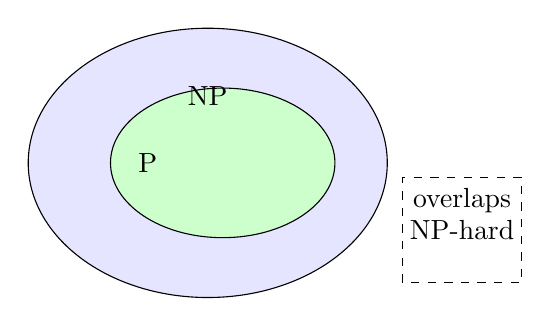
\begin{tikzpicture}[scale=0.95]
    \draw[fill=blue!10] (0,0) ellipse (2.4cm and 1.8cm);
    \draw[fill=green!20] (0.2,0) ellipse (1.5cm and 1cm);
    \node at (0,0.9) {NP};
    \node at (-0.8,0) {P};
    \draw[dashed] (2.6,-1.6) rectangle (4.2,-0.2);
    \node at (3.4,-0.9) {NP-hard};
    \node at (3.4,-0.5) {overlaps};
  \end{tikzpicture}
  \end{center}
  \begin{itemize}
    \item P sits inside NP
    \item NP-complete problems are the hard core inside NP
  \end{itemize}
\end{frame}

\begin{frame}{Famous Examples}
  \begin{center}
  \begin{tabular}{ll}
    \toprule
    Problem & Class \\
    \midrule
    Sorting & P \\
    Shortest path & P \\
    2-colorability & P \\
    3-SAT & NP-complete \\
    Clique & NP-complete \\
    Hamiltonian cycle & NP-complete \\
    TSP decision version & NP-complete \\
    \bottomrule
  \end{tabular}
  \end{center}
\end{frame}

\begin{frame}{Why Optimization Is Often Harder to State}
  \begin{itemize}
    \item "find the best" usually turns into a search over many possibilities
    \item decision form often captures the same hardness more cleanly
    \item optimization can be NP-hard even when the decision version is NP-complete
  \end{itemize}
  \begin{exampleblock}{Example}
    "Is there a schedule with at most $k$ conflicts?" is easier to classify than "find the schedule with minimum conflicts."
  \end{exampleblock}
\end{frame}

\begin{frame}{P Versus NP}
  \begin{alertblock}{The question}
    Does every problem whose answer can be checked quickly also have a quick algorithm for finding the answer?
  \end{alertblock}
  \begin{itemize}
    \item this is the famous P vs NP question
    \item it remains open
    \item most computer scientists believe P $\ne$ NP
  \end{itemize}
\end{frame}

\begin{frame}{Practical Meaning of NP-Hardness}
  \begin{itemize}
    \item do not expect a polynomial-time exact algorithm in the general case
    \item use heuristics, approximation, or special-case structure
    \item exploit domain constraints whenever possible
  \end{itemize}
  \begin{block}{Engineering response}
    The right question is often "what kind of answer do we need, and how good does it need to be?"
  \end{block}
\end{frame}

\begin{frame}{A Campus Scheduling Example}
  \begin{itemize}
    \item rooms have limited capacity
    \item classes cannot overlap for the same students
    \item teachers have availability constraints
  \end{itemize}
  \begin{alertblock}{Why this is hard}
    The number of feasible combinations grows very quickly.
  \end{alertblock}
\end{frame}

\begin{frame}{Certificates and Verifiers in Practice}
  \begin{itemize}
    \item a certificate is a candidate schedule
    \item the verifier checks room sizes, time clashes, and teacher constraints
    \item checking is much easier than searching
  \end{itemize}
  \begin{exampleblock}{This is the NP pattern}
    Quick verification does not imply quick discovery.
  \end{exampleblock}
\end{frame}

\section{Reductions}
\begin{frame}{What Is a Reduction?}
  \begin{itemize}
    \item transform instances of problem A into instances of problem B
    \item preserve the answer
    \item use B as a solver for A
  \end{itemize}
  \begin{block}{Intuition}
    If A can be turned into B quickly, then B is at least as hard as A.
  \end{block}
\end{frame}

\begin{frame}{Reduction Template}
  \begin{enumerate}
    \item start with an instance of A
    \item encode it as an instance of B
    \item prove the encoding is polynomial-time
    \item prove yes instances map to yes instances and no instances map to no instances
  \end{enumerate}
\end{frame}

\begin{frame}{Why Reductions Matter}
  \begin{itemize}
    \item they let us compare problem hardness
    \item they let us reuse known hardness results
    \item they explain why many different problems share the same difficulty
  \end{itemize}
  \begin{exampleblock}{In one sentence}
    Reductions are the bridge between new problems and known hard problems.
  \end{exampleblock}
\end{frame}

\begin{frame}{Example Reduction Pattern}
  \begin{itemize}
    \item identify the hard structure inside the new problem
    \item map items to vertices, constraints to edges, or clauses to gadgets
    \item preserve satisfiability or feasibility
  \end{itemize}
  \begin{block}{Common idea}
    Encode logical constraints into a combinatorial object.
  \end{block}
\end{frame}

\begin{frame}{Vertex Cover and Independent Set}
  \begin{itemize}
    \item a vertex cover touches every edge
    \item an independent set contains no edge
    \item the two notions are complementary
  \end{itemize}
  \begin{exampleblock}{Reduction idea}
    A graph has an independent set of size $k$ if and only if it has a vertex cover of size $|V|-k$.
  \end{exampleblock}
\end{frame}

\begin{frame}{SAT as a Hardness Source}
  \begin{itemize}
    \item Boolean satisfiability is the canonical NP-complete problem
    \item many reductions start from SAT or 3-SAT
    \item clauses become gadgets or structural constraints
  \end{itemize}
  \begin{block}{Why SAT matters}
    Once SAT is hard, many other problems inherit hardness through reductions.
  \end{block}
\end{frame}

\begin{frame}{3-SAT and Clique}
  \begin{itemize}
    \item variables and clauses can be encoded as graph vertices
    \item compatible choices become edges
    \item a clique represents a consistent selection
  \end{itemize}
  \begin{alertblock}{Conceptual takeaway}
    Reduction proofs are about preserving structure, not just translating words.
  \end{alertblock}
\end{frame}

\begin{frame}{How to Read a Reduction Proof}
  \begin{itemize}
    \item look for the source problem and the target problem
    \item identify the mapping
    \item check both directions of correctness
    \item check the time required for the transformation
  \end{itemize}
  \begin{block}{Checklist}
    Source, target, transformation, correctness, complexity.
  \end{block}
\end{frame}

\begin{frame}{Common Reduction Mistakes}
  \begin{itemize}
    \item proving only one direction
    \item forgetting the polynomial-time requirement
    \item confusing optimization with decision form
    \item assuming the reduction itself is the algorithm
  \end{itemize}
  \begin{alertblock}{Warning}
    A reduction does not solve the problem. It only relates it to another one.
  \end{alertblock}
\end{frame}

\begin{frame}{Approximation and Heuristics}
  \begin{itemize}
    \item exact solutions may be too expensive
    \item approximation algorithms give provable near-optimal answers
    \item heuristics give practical answers without a formal guarantee
  \end{itemize}
  \begin{exampleblock}{Engineering lesson}
    For hard problems, good enough can be the right goal.
  \end{exampleblock}
\end{frame}

\begin{frame}{A Decision Version Example}
  \begin{itemize}
    \item optimization: find the smallest number of rooms
    \item decision: is there a schedule using at most $k$ rooms?
    \item the decision version is often the one used in complexity theory
  \end{itemize}
  \begin{block}{Why}
    Decision problems fit clean yes/no verification.
  \end{block}
\end{frame}

\begin{frame}{Reduction Strategy for Exams}
  \begin{enumerate}
    \item identify a known NP-complete problem
    \item map its instances to the new problem
    \item prove the mapping preserves yes/no answers
    \item explain why the mapping is polynomial
  \end{enumerate}
\end{frame}

\section{Undecidability and Limits}
\begin{frame}{Decidable and Undecidable}
  \begin{itemize}
    \item a decidable problem has an algorithm that always halts with the correct answer
    \item an undecidable problem has no such algorithm
  \end{itemize}
  \begin{block}{Example}
    Connectivity is decidable. The halting problem is not.
  \end{block}
\end{frame}

\begin{frame}{The Halting Problem}
  \begin{alertblock}{Question}
    Given a program $P$ and input $I$, will $P$ eventually halt?
  \end{alertblock}
  \begin{itemize}
    \item Turing proved that no algorithm can solve this for all programs and inputs
    \item this is one of the foundational limits of computation
  \end{itemize}
\end{frame}

\begin{frame}{Why This Matters for Software}
  \begin{itemize}
    \item there is no perfect general-purpose bug detector
    \item there is no general method that proves every program halts
    \item static analysis and testing are useful, but they are not omniscient
  \end{itemize}
  \begin{exampleblock}{Practical meaning}
    Some questions are not just hard; they are impossible to solve in full generality.
  \end{exampleblock}
\end{frame}

\begin{frame}{Semi-Decidable Problems}
  \begin{itemize}
    \item some problems have algorithms that halt on yes instances
    \item they may run forever on no instances
    \item this is weaker than decidability
  \end{itemize}
  \begin{block}{Use}
    Semi-decidability appears in theorem proving and search over infinite spaces.
  \end{block}
\end{frame}

\begin{frame}{Diagonalisation Idea}
  \begin{itemize}
    \item assume a perfect halting checker exists
    \item build a program that contradicts the checker on itself
    \item the contradiction shows the checker cannot exist
  \end{itemize}
  \begin{alertblock}{Method}
    This proof style is one of the classic tools for impossibility results.
  \end{alertblock}
\end{frame}

\begin{frame}{Limits and Boundaries}
  \begin{itemize}
    \item P, NP, NP-hard, and undecidable are different kinds of difficulty
    \item "hard" does not always mean the same thing
    \item choose the right language for the right limit
  \end{itemize}
  \begin{block}{Summary}
    Some problems are slow. Some are search-hard. Some are impossible to decide.
  \end{block}
\end{frame}

\section{Exercise Walkthroughs}
\begin{frame}{Exercise 2.1: Proofs by Definition}
  \begin{itemize}
    \item $5n^2 + 3n = O(n^2)$
    \item $n^2/4 = \Omega(n)$
    \item $3n\log n + n = \Theta(n\log n)$
    \item $\log_2 n = \Theta(\log_{10} n)$
  \end{itemize}
  \begin{block}{What to do}
    Write the constants explicitly and show the inequalities for large enough $n$.
  \end{block}
\end{frame}

\begin{frame}{Exercise 2.2: Ordering Growth Rates}
  \begin{itemize}
    \item compare $\sqrt n$, $\log^2 n$, $n\log n$, $n^{1.5}$, $n^2$, $2^n$, $3^n$, and $n!$
    \item use the growth ladder rather than raw calculation
  \end{itemize}
  \begin{exampleblock}{Expected pattern}
    logarithmic, root, linear-log, fractional polynomial, quadratic, exponential, factorial
  \end{exampleblock}
\end{frame}

\begin{frame}{Exercise 2.3: Sums and Dominant Terms}
  \begin{itemize}
    \item $\sum_{i=1}^{n} i^2$
    \item $\sum_{i=1}^{\log n} n$
    \item $\sum_{i=0}^{n} 2^i$
    \item $n^2 2^n + n^{100}$
  \end{itemize}
  \begin{block}{Strategy}
    Use standard sum formulas and keep the dominant term.
  \end{block}
\end{frame}

\begin{frame}{Exercise 2.4: Properties}
  \begin{itemize}
    \item $f(n)=O(g(n)) \Rightarrow g(n)=\Omega(f(n))$
    \item $f(n)+g(n)=\Theta(\max(f(n),g(n)))$
    \item if $f=O(g)$ and $g=O(h)$, then $f g = O(h^2)$
  \end{itemize}
  \begin{block}{Use}
    These are algebraic tools, but every claim still needs justification.
  \end{block}
\end{frame}

\begin{frame}{Exercise 2.5: Loop Complexity}
  \begin{itemize}
    \item nested doubling loops
    \item recursive split-and-combine recurrence
    \item unusual inner step sizes
  \end{itemize}
  \begin{exampleblock}{What to look for}
    Count the number of iterations per outer loop and convert to a sum or recurrence.
  \end{exampleblock}
\end{frame}

\begin{frame}{Exercise 2.6: Space Complexity}
  \begin{itemize}
    \item recursive factorial: stack frames grow with $n$
    \item iterative factorial: constant extra space
    \item recursive binary search: $O(\log n)$ stack space
    \item iterative binary search: $O(1)$ extra space
  \end{itemize}
\end{frame}

\begin{frame}{Exercise 2.7: Classify Problems}
  \begin{itemize}
    \item sorting, shortest path, bipartite check: P
    \item 3-SAT, clique, Hamiltonian cycle: NP-complete
    \item graph coloring with 3 colors: NP-complete
    \item Eulerian circuit: P
  \end{itemize}
  \begin{block}{Reminder}
    Always say whether you mean the decision or optimization version.
  \end{block}
\end{frame}

\begin{frame}{Exercise 2.8: The Halting Problem}
  \begin{itemize}
    \item state the problem in terms of a program and input
    \item explain the diagonal argument at a high level
    \item connect the result to software limits
  \end{itemize}
\end{frame}

\begin{frame}{Exercise 2.9: Reductions in Your Own Words}
  \begin{itemize}
    \item explain what it means to transform instances of one problem into another
    \item explain why a polynomial reduction preserves hardness
  \end{itemize}
  \begin{block}{Core sentence}
    If a known hard problem reduces to a new problem, the new problem is at least as hard.
  \end{block}
\end{frame}

\begin{frame}{Challenge 2.10}
  \begin{itemize}
    \item prove $\sum_{k=1}^{n} k = \Theta(n^2)$
    \item find explicit constants
  \end{itemize}
  \begin{exampleblock}{Hint}
    Use the closed form $n(n+1)/2$ and compare it to $n^2$.
  \end{exampleblock}
\end{frame}

\begin{frame}{Challenge 2.11}
  \begin{itemize}
    \item if $f(n)=o(g(n))$, then $f(n)=O(g(n))$
    \item but then $f(n)\neq \Theta(g(n))$
  \end{itemize}
  \begin{block}{Hint}
    The ratio $f(n)/g(n)$ is the key object.
  \end{block}
\end{frame}

\begin{frame}{Challenge 2.12}
  \begin{itemize}
    \item integer sorting with van Emde Boas trees
    \item range size $U$ matters
    \item compare the dependence on $U$ with comparison sorting lower bounds
  \end{itemize}
  \begin{alertblock}{Research angle}
    The data structure can beat comparison sorting only when the key universe is structured enough.
  \end{alertblock}
\end{frame}

\section{Advanced Problems and Further Reading}
\begin{frame}{Advanced Topic: Average Case Versus Worst Case}
  \begin{itemize}
    \item worst-case analysis is robust
    \item average-case analysis depends on an input model
    \item randomized algorithms mix both ideas
  \end{itemize}
  \begin{block}{Why it matters}
    A slow worst case does not always mean a bad practical algorithm, but the assumption must be explicit.
  \end{block}
\end{frame}

\begin{frame}{Advanced Topic: Fine-Grained Complexity}
  \begin{itemize}
    \item not all polynomial algorithms are equally good
    \item $n^{2}$ and $n^{1.5}$ can be meaningfully different in practice
    \item fine-grained complexity studies the exact exponent and small improvements
  \end{itemize}
\end{frame}

\begin{frame}{Advanced Topic: Approximation}
  \begin{itemize}
    \item exact optimization may be NP-hard
    \item approximation gives a provable near-optimal answer
    \item this is often the right tool for real systems
  \end{itemize}
  \begin{exampleblock}{Campus example}
    A near-optimal exam schedule can be much better than no schedule at all.
  \end{exampleblock}
\end{frame}

\begin{frame}{Advanced Topic: Randomization}
  \begin{itemize}
    \item randomness can simplify algorithms
    \item randomized quicksort is a classic example
    \item the analysis uses expected cost
  \end{itemize}
  \begin{block}{Preview}
    Week 14 will return to this idea in more depth.
  \end{block}
\end{frame}

\begin{frame}{Practical Break-Even Points}
  \begin{itemize}
    \item asymptotics explain the far end of the curve
    \item real systems also need a break-even point
    \item a slower asymptotic algorithm can win on tiny inputs
  \end{itemize}
  \begin{exampleblock}{Engineering habit}
    Always ask both "what is the growth class?" and "where does the crossover happen?"
  \end{exampleblock}
\end{frame}

\begin{frame}{Quick Formula Sheet}
  \begin{itemize}
    \item $f(n)=O(g(n))$: upper bound
    \item $f(n)=\Omega(g(n))$: lower bound
    \item $f(n)=\Theta(g(n))$: tight bound
    \item $f(n)=o(g(n))$: strictly smaller growth
  \end{itemize}
\end{frame}

\begin{frame}{One Worked Comparison}
  Compare these two costs:
  \[
    A(n)=3n^2+40n+17,\qquad B(n)=1000n
  \]
  \begin{itemize}
    \item $A(n)$ is $\Theta(n^2)$
    \item $B(n)$ is $\Theta(n)$
    \item the linear algorithm wins eventually
  \end{itemize}
\end{frame}

\begin{frame}{Study Checklist}
  \begin{itemize}
    \item can you state each definition from memory?
    \item can you prove one upper bound and one lower bound?
    \item can you rank the standard growth families?
    \item can you explain P, NP, NP-complete, and NP-hard in one sentence each?
  \end{itemize}
\end{frame}

\begin{frame}{Further Reading}
  \begin{itemize}
    \item CLRS, Chapter 3 and Appendix on complexity
    \item Jeff Erickson, \emph{Algorithms}
    \item Complexity Zoo: \url{https://complexityzoo.net/}
    \item MIT OCW 6.006 lectures on asymptotic analysis
  \end{itemize}
\end{frame}

\begin{frame}{Week 2 Summary}
  \begin{enumerate}
    \item Big-O gives an upper bound
    \item Big-Omega gives a lower bound
    \item Big-Theta gives a tight bound
    \item proofs need constants and a threshold
    \item growth classes separate linear, polynomial, exponential, and factorial behavior
    \item P, NP, NP-complete, NP-hard, and undecidable are different notions of difficulty
    \item reductions are the main tool for comparing problem hardness
  \end{enumerate}
\end{frame}

\begin{frame}{Next Week}
  \begin{itemize}
    \item divide and conquer
    \item merge sort
    \item quick sort
    \item recurrence relations
  \end{itemize}
  \begin{block}{Preparation}
    Review the growth ladder and the proof patterns before moving to recurrences.
  \end{block}
\end{frame}

\begin{frame}{Discussion Prompts}
  \begin{itemize}
    \item Which part of algorithm analysis feels most mechanical?
    \item Which part feels easiest to get wrong?
    \item Which problem class would matter most in a student-information system?
  \end{itemize}
\end{frame}

\end{document}
